\section{Register description}
\regover{
{\hyperref[cam-cam-dvp2axi-configue]{cam\_dvp2axi\_configue}}&Camera configure
\\
\hline
{\hyperref[cam-cam-dvp2axi-addr-start]{cam\_dvp2axi\_addr\_start}}&Start of write address
\\
\hline
{\hyperref[cam-cam-dvp2axi-mem-bcnt]{cam\_dvp2axi\_mem\_bcnt}}&Burst count of memory
\\
\hline
{\hyperref[cam-cam-dvp-status-and-error]{cam\_dvp\_status\_and\_error}}&Interrupt and bus status
\\
\hline
{\hyperref[cam-cam-dvp2axi-frame-bcnt]{cam\_dvp2axi\_frame\_bcnt}}&Byte count of frame
\\
\hline
{\hyperref[cam-cam-dvp-frame-fifo-pop]{cam\_dvp\_frame\_fifo\_pop}}&Interrupt clear and pop
\\
\hline
{\hyperref[cam-cam-dvp2axi-frame-vld]{cam\_dvp2axi\_frame\_vld}}&Frame valid in period
\\
\hline
{\hyperref[cam-cam-dvp2axi-frame-period]{cam\_dvp2axi\_frame\_period}}&Frame period
\\
\hline
{\hyperref[cam-cam-dvp2axi-misc]{cam\_dvp2axi\_misc}}&RGB565 and RGBA8888 setting
\\
\hline
{\hyperref[cam-cam-dvp2axi-hsync-crop]{cam\_dvp2axi\_hsync\_crop}}&Hsync crop
\\
\hline
{\hyperref[cam-cam-dvp2axi-vsync-crop]{cam\_dvp2axi\_vsync\_crop}}&Vsync crop
\\
\hline
{\hyperref[cam-cam-dvp2axi-fram-exm]{cam\_dvp2axi\_fram\_exm}}&Total valid count
\\
\hline
{\hyperref[cam-cam-frame-start-addr0]{cam\_frame\_start\_addr0}}&Start address of frame0
\\
\hline
{\hyperref[cam-cam-frame-start-addr1]{cam\_frame\_start\_addr1}}&Start address of frame1
\\
\hline
{\hyperref[cam-cam-frame-start-addr2]{cam\_frame\_start\_addr2}}&Start address of frame2
\\
\hline
{\hyperref[cam-cam-frame-start-addr3]{cam\_frame\_start\_addr3}}&Start address of frame3
\\
\hline
{\hyperref[cam-cam-frame-id-sts01]{cam\_frame\_id\_sts01}}&ID of frame 0/1
\\
\hline
{\hyperref[cam-cam-frame-id-sts23]{cam\_frame\_id\_sts23}}&ID of frame 2/3
\\
\hline
{\hyperref[cam-cam-dvp-debug]{cam\_dvp\_debug}}&ID latch timing
\\
\hline
}

\subsection{cam\_dvp2axi\_configue}
\label{cam-cam-dvp2axi-configue}
Address:0x20057000
 \begin{figure}[H]
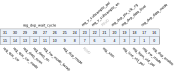
\includegraphics{cam_cam_dvp2axi_configue.pdf}
\end{figure}

\regdes{31:24&reg\_dvp\_wait\_cycle&r/w&8'h40&Cycles in FSM Wait mode\\\hline
23&reg\_v\_subsample\_pol&r/w&1'b0&DVP2BUS vertical sub-sampling polarity \par 1'b0: Odd lines are masked \par 1'b1: Even lines are masked
\\\hline
22&reg\_v\_subsample\_en&r/w&1'b0&DVP2BUS vertical sub-sampling enable\\\hline
21&RSVD& & & \\\hline
20&reg\_dvp\_pix\_clk\_cg&r/w&1'b0&DVP pix clk gate\\\hline
19&reg\_dvp\_data\_bsel&r/w&1'b0&Byte select signal for DVP 8-bit mode, don't care if reg\_dvp\_data\_8bit is disabled \par 1'b0: Select the lower byte of pix\_data \par 1'b1: Select the upper byte of pix\_data
\\\hline
18:16&reg\_dvp\_data\_mode&r/w&3'b0&DVP 8-bit mode enable \par 3'd0: DVP pix\_data is 16-bit wide \par 3'd1: DVP pix\_data is 24-bit mode \par 3'd2: DVP pix\_data is 24-comp-16-bit mode \par 3'd3: DVP pix\_data is 24-exp-32-bit mode \par 3'd4: DVP pix\_data is 8-bit wide \par Others - Reserved
\\\hline
15&reg\_qos\_sw&r/w&1'b0&AXI Qos software mode value\\\hline
14&reg\_qos\_sw\_mode&r/w&1'b0&AXI QoS software mode enable\\\hline
13&reg\_drop\_even&r/w&1'b0&Only effect when reg\_drop\_en=1 :  \par 1'b1 : Drop all even bytes \par 1'b0 : Drop all odd bytes
\\\hline
12&reg\_drop\_en&r/w&1'b0&Drop mode Enable\\\hline
11&reg\_hw\_mode\_fwrap&r/w&1'b1&DVP2BUS HW mode with frame start address wrap to reg\_addr\_start\\\hline
10:8&reg\_dvp\_mode&r/w&3'd0&Image senosr mode selection:  \par 3'd0-Vsync\&Hsync \par 3'd1-Vsync|Hsync \par 3'd2-Vsync \par 3'd3-Hsync
\\\hline
7&RSVD& & & \\\hline
6:4&reg\_xlen&r/w&3'd3&burst length setting  \par 3'd0 - Single / 3'd1 - INCR4 / 3'd2 - INCR8 \par 3'd3 - INCR16 / 3'd5 - INCR32 / 3'd6 - INCR64
\\\hline
3&reg\_line\_vld\_pol&r/w&1'b1&Image sensor line valid polarity, 1'b0 - Activel low, 1'b1 - Active high\\\hline
2&reg\_fram\_vld\_pol&r/w&1'b1&Image sensor frame valid polarity, 1'b0 - Activel low, 1'b1 - Active high\\\hline
1&reg\_sw\_mode&r/w&1'b0&DVP2BUS SW manual mode (don't care if reg\_swap\_mode is enabled)\\\hline
0&reg\_dvp\_enable&r/w&1'b0&module enable\\\hline

}
\subsection{cam\_dvp2axi\_addr\_start}
\label{cam-cam-dvp2axi-addr-start}
Address:0x20057004
 \begin{figure}[H]
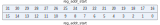
\includegraphics{cam_cam_dvp2axi_addr_start.pdf}
\end{figure}

\regdes{31:0&reg\_addr\_start&r/w&32'h80000000&AXI start address\\\hline

}
\subsection{cam\_dvp2axi\_mem\_bcnt}
\label{cam-cam-dvp2axi-mem-bcnt}
Address:0x20057008
 \begin{figure}[H]
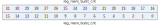
\includegraphics{cam_cam_dvp2axi_mem_bcnt.pdf}
\end{figure}

\regdes{31:0&reg\_mem\_burst\_cnt&r/w&32'hC000&AXI burst cnt before wrap to "reg\_addr\_start"\\\hline

}
\subsection{cam\_dvp\_status\_and\_error}
\label{cam-cam-dvp-status-and-error}
Address:0x2005700c
 \begin{figure}[H]
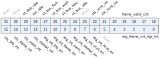
\includegraphics{cam_cam_dvp_status_and_error.pdf}
\end{figure}

\regdes{31:30&RSVD& & & \\\hline
29&st\_dvp\_idle&r&1'b1&DVP2BUS asynchronous fifo idle status\\\hline
28&axi\_idle&r&1'b1&DVP2BUS AHB idle status\\\hline
27&st\_bus\_flsh&r&1'b0&DVP in flush state\\\hline
26&st\_bus\_wait&r&1'b0&DVP in wait state\\\hline
25&st\_bus\_func&r&1'b0&DVP in functional state\\\hline
24&st\_bus\_idle&r&1'b1&DVP in idle state\\\hline
23&RSVD& & & \\\hline
22&sts\_vcnt\_int&r&1'b0&Vsync valid line count non-match interrupt status\\\hline
21&sts\_hcnt\_int&r&1'b0&Hsync valid pixel count non-match interrupt status\\\hline
20:16&frame\_valid\_cnt&r&5'd0&Frame counts in memory before read out in SW mode\\\hline
15&sts\_fifo\_int&r&1'b0&FIFO OverWrite interrupt status\\\hline
14&sts\_frame\_int&r&1'b0&Frame OverWrite interrupt status\\\hline
13&sts\_mem\_int&r&1'b0&Memory OverWrite interrupt status\\\hline
12&sts\_normal\_int&r&1'b0&Normal Write interrupt status\\\hline
11&reg\_int\_fifo\_en&r/w&1'b1&FIFO OverWrite interrupt enable\\\hline
10&reg\_int\_frame\_en&r/w&1'b0&Frame OverWrite interrupt enable\\\hline
9&reg\_int\_mem\_en&r/w&1'b0&Memory OverWrite interrupt enable\\\hline
8&reg\_int\_normal\_en&r/w&1'b0&Normal Write interrupt enable\\\hline
7&reg\_int\_vcnt\_en&r/w&1'b0&Vsync valid line count match interrupt enable\\\hline
6&reg\_int\_hcnt\_en&r/w&1'b0&Hsync valid pixel count match interrupt enable\\\hline
5&RSVD& & & \\\hline
4:0&reg\_frame\_cnt\_trgr\_int&r/w&5'd0&Frame to issue interrupt at SW Mode\\\hline

}
\subsection{cam\_dvp2axi\_frame\_bcnt}
\label{cam-cam-dvp2axi-frame-bcnt}
Address:0x20057010
 \begin{figure}[H]
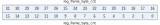
\includegraphics{cam_cam_dvp2axi_frame_bcnt.pdf}
\end{figure}

\regdes{31:0&reg\_frame\_byte\_cnt&r/w&32'h7e90&Single Frame byte cnt(Need pre-calculation)\\\hline

}
\subsection{cam\_dvp\_frame\_fifo\_pop}
\label{cam-cam-dvp-frame-fifo-pop}
Address:0x20057014
 \begin{figure}[H]
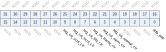
\includegraphics{cam_cam_dvp_frame_fifo_pop.pdf}
\end{figure}

\regdes{31:10&RSVD& & & \\\hline
9&reg\_int\_vcnt\_clr&w1p&1'd0&Interrupt clear\\\hline
8&reg\_int\_hcnt\_clr&w1p&1'd0&Interrupt clear\\\hline
7&reg\_int\_fifo\_clr&w1p&1'd0&Interrupt clear\\\hline
6&reg\_int\_frame\_clr&w1p&1'd0&Interrupt clear\\\hline
5&reg\_int\_mem\_clr&w1p&1'd0&Interrupt clear\\\hline
4&reg\_int\_normal\_clr&w1p&1'd0&Interrupt clear\\\hline
3:1&RSVD& & & \\\hline
0&rfifo\_pop&w1p&1'b0&Write this bit will trigger fifo pop\\\hline

}
\subsection{cam\_dvp2axi\_frame\_vld}
\label{cam-cam-dvp2axi-frame-vld}
Address:0x20057018
 \begin{figure}[H]
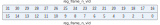
\includegraphics{cam_cam_dvp2axi_frame_vld.pdf}
\end{figure}

\regdes{31:0&reg\_frame\_n\_vld&r/w&32'hffff\_ffff&Bitwise frame valid in period\\\hline

}
\subsection{cam\_dvp2axi\_frame\_period}
\label{cam-cam-dvp2axi-frame-period}
Address:0x2005701c
 \begin{figure}[H]
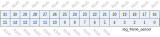
\includegraphics{cam_cam_dvp2axi_frame_period.pdf}
\end{figure}

\regdes{31:5&RSVD& & & \\\hline
4:0&reg\_frame\_period&r/w&5'h0&Frame period cnt. (EX. Set this register 0, the period is 1)\\\hline

}
\subsection{cam\_dvp2axi\_misc}
\label{cam-cam-dvp2axi-misc}
Address:0x20057020
 \begin{figure}[H]
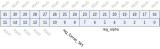
\includegraphics{cam_cam_dvp2axi_misc.pdf}
\end{figure}

\regdes{31:11&RSVD& & & \\\hline
10:8&reg\_format\_565&r/w&3'd0&Only work when reg\_dvp\_data\_mode=2 (24-comp-16-bit mode) \par 3'd0: B2(5)B1(6)B0(5) \par 3'd1: B1(5)B2(6)B0(5) \par 3'd2: B2(5)B0(6)B1(5) \par 3'd3: B0(5)B2(6)B1(5) \par 3'd4: B1(5)B0(6)B2(5) \par 3'd5: B0(5)B1(6)B2(5)
\\\hline
7:0&reg\_alpha&r/w&8'h0&Only work when "reg\_dvp\_data\_mode==2'd3(DVP pix\_data is 24-exp-32-bit mode)" \par The value of [31:24]
\\\hline

}
\subsection{cam\_dvp2axi\_hsync\_crop}
\label{cam-cam-dvp2axi-hsync-crop}
Address:0x20057030
 \begin{figure}[H]
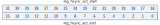
\includegraphics{cam_cam_dvp2axi_hsync_crop.pdf}
\end{figure}

\regdes{31:16&reg\_hsync\_act\_start&r/w&16'h0&Valid hsync start cnt\\\hline
15:0&reg\_hsync\_act\_end&r/w&16'hFFFF&Valid hsync end cnt\\\hline

}
\subsection{cam\_dvp2axi\_vsync\_crop}
\label{cam-cam-dvp2axi-vsync-crop}
Address:0x20057034
 \begin{figure}[H]
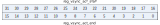
\includegraphics{cam_cam_dvp2axi_vsync_crop.pdf}
\end{figure}

\regdes{31:16&reg\_vsync\_act\_start&r/w&16'h0&Valid vsync start cnt\\\hline
15:0&reg\_vsync\_act\_end&r/w&16'hFFFF&Valid vsync end cnt\\\hline

}
\subsection{cam\_dvp2axi\_fram\_exm}
\label{cam-cam-dvp2axi-fram-exm}
Address:0x20057038
 \begin{figure}[H]
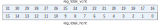
\includegraphics{cam_cam_dvp2axi_fram_exm.pdf}
\end{figure}

\regdes{31:16&reg\_total\_vcnt&r/w&16'h0&Total valid line count in a frame\\\hline
15:0&reg\_total\_hcnt&r/w&16'h0&Total valid pix count in a line\\\hline

}
\subsection{cam\_frame\_start\_addr0}
\label{cam-cam-frame-start-addr0}
Address:0x20057040
 \begin{figure}[H]
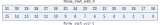
\includegraphics{cam_cam_frame_start_addr0.pdf}
\end{figure}

\regdes{31:0&frame\_start\_addr\_0&r&32'd0&DVP2BUS PIC 0 Start address\\\hline

}
\subsection{cam\_frame\_start\_addr1}
\label{cam-cam-frame-start-addr1}
Address:0x20057048
 \begin{figure}[H]
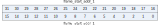
\includegraphics{cam_cam_frame_start_addr1.pdf}
\end{figure}

\regdes{31:0&frame\_start\_addr\_1&r&32'd0&DVP2BUS PIC 1 Start address\\\hline

}
\subsection{cam\_frame\_start\_addr2}
\label{cam-cam-frame-start-addr2}
Address:0x20057050
 \begin{figure}[H]
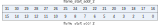
\includegraphics{cam_cam_frame_start_addr2.pdf}
\end{figure}

\regdes{31:0&frame\_start\_addr\_2&r&32'd0&DVP2BUS PIC 2 Start address\\\hline

}
\subsection{cam\_frame\_start\_addr3}
\label{cam-cam-frame-start-addr3}
Address:0x20057058
 \begin{figure}[H]
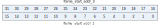
\includegraphics{cam_cam_frame_start_addr3.pdf}
\end{figure}

\regdes{31:0&frame\_start\_addr\_3&r&32'd0&DVP2BUS PIC 3 Start address\\\hline

}
\subsection{cam\_frame\_id\_sts01}
\label{cam-cam-frame-id-sts01}
Address:0x20057060
 \begin{figure}[H]
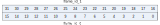
\includegraphics{cam_cam_frame_id_sts01.pdf}
\end{figure}

\regdes{31:16&frame\_id\_1&r&16'd0&DVP2BUS PIC 1 ID\\\hline
15:0&frame\_id\_0&r&16'd0&DVP2BUS PIC 0 ID\\\hline

}
\subsection{cam\_frame\_id\_sts23}
\label{cam-cam-frame-id-sts23}
Address:0x20057064
 \begin{figure}[H]
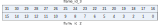
\includegraphics{cam_cam_frame_id_sts23.pdf}
\end{figure}

\regdes{31:16&frame\_id\_3&r&16'd0&DVP2BUS PIC 3 ID\\\hline
15:0&frame\_id\_2&r&16'd0&DVP2BUS PIC 2 ID\\\hline

}
\subsection{cam\_dvp\_debug}
\label{cam-cam-dvp-debug}
Address:0x200570f0
 \begin{figure}[H]
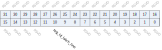
\includegraphics{cam_cam_dvp_debug.pdf}
\end{figure}

\regdes{31:12&RSVD& & & \\\hline
11:8&reg\_id\_latch\_line&r/w&4'd5&ID latch timing (line count)\\\hline
7:32&RSVD& & & \\\hline
31:0&RESERVED&rsvd&32'hf0f0f0f0&RESERVED\\\hline

}
